%ANI: The title of the report - Twitter as an alternative review site -> Twitter as an Alternative Review Site
%ANI: recommender -> recommender system. Also fix previous mentions.

\chapter{Introduction}

\section{Twitter as a Source of Reviews}
The rapid development and expansion of the internet has introduced new ways for individuals to express their opinions and disseminate their views. Online reviews have become a hugely important source of information for consumers. They play an important role in determining whether a person is satisfied with a product or service. Online reviews provide a huge amount of data on consumer preferences. It is now relatively rare that someone will purchase a product, reserve a table at a restaurant or book a room in a hotel without first checking some online reviews. These reviews inform and influence consumer decisions, and have a direct relationship with online sales. 

This project will focus on Twitter, a microblogging social media site, where users can post short blocks of text of no more than 280 characters. Twitter currently has ~126 million people who use the site daily, which the company terms `monetizable Daily Active Users' (mDAU), with over 500 million tweets posted per day \cite{Twitter2019}. These tweets can often take the form of a review (Figure ~\ref{fig:tweets}).

\begin{figure}[h!]
\centering
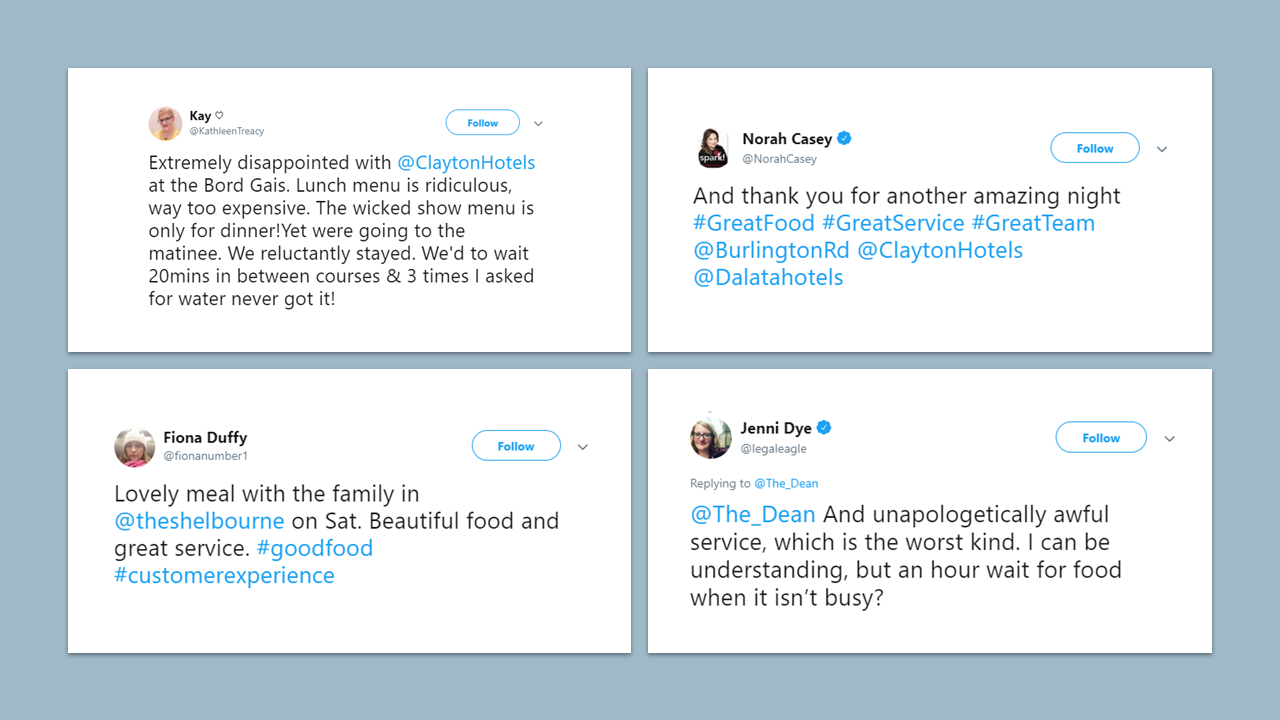
\includegraphics[width=1\textwidth]{introduction/sample_tweets.png}
\caption{\label{fig:tweets} Examples of Review-like Tweets.}
\end{figure}

Twitter users post tweets which express their ideas and opinions on a wide array of topics. An individual may, for example, tweet about a city they visited, a hotel they stayed in, a restaurant they ate at or a film they watched. These review-like tweets can give insight into consumers' opinions on the entities with which they interact. With millions of tweets being posted every day, Twitter has a huge potential source of underutilised reviews.

Traditional online review sites include websites like Tripadvisor, Foursquare and Yelp. Often these sites have a dedicated area for feedback and encourage users to leave reviews of their hotels, restaurants or products. In our opinion this method of obtaining reviews can sometimes result in more forced, manufactured, less reliable reviews. It is our contention that users tend to post their genuine feelings more spontaneously and frequently to Twitter. Users often wouldn't consider their posts to be a 'review' in the formal sense of the word and not in the same way they would consider a review left in the dedicated feedback area of another website.

%SL: also because they probably don't consider their posts to be a 'review' in the formal sense of the word
%SL: One note of caution here, unless you can find research papers which back up the assertions here - more spontaneous posting, forced reviews on reviews on review sites, more honest reviews on twitter - then we need to make clear that this is our contention/opinion/assumptions. If you can find papers to back it up, you should reference them here. Ani may have suitable references from his PhD work  
%ANI: Yes, we need to be careful here. I think terms such as spontaneous and unfiltered are fine to use. These reviews are different. We do not want to claim that these review-like tweets are better (source of information) than other on-line reviews available from sites such as Foursquare, Yelp until we can show by experiments.

The language used in tweets is different to longer form text and needs to be treated differently. Tweets are usually very informal, using casual language and slang. They contain things like hashtags, emojis, twitter handles, URLs, images, videos and gifs.

\section{Research Question}
This research project will investigate how useful Twitter can be when used as an alternative or additional source of reviews for use in a recommender system. We will explore methods of classifying review-like tweets, identifying the sentiment of the reviews and the effect of using this data in a recommender system.

The following research question will be addressed:
\begin{center}
\textbf{To what extent can Twitter provide a suitable source of online reviews that can be used effectively in the generation of recommendations in a recommender system?}
\end{center}

\section{Research Objectives}
The project will focus on tweets that mention or discuss hotels in the Dublin area. A collection of 2.5 million tweets posted from Dublin, collected between October 2017 and September 2018, will be used as the dataset. The main objective of the project is to determine whether tweets can be used successfully as a source of reviews in a recommender system.

The objectives of this research project are:
\begin{enumerate}
%ANI: You may want to add "Data Collection" as the first step where you can describe how you collected the data. Which Twitter API (Search/Streaming) has been used? Describe that you set a geographic bounding box over Dublin to collect all the tweets that are coming from within that bounding box. etc.
    \item \textbf{Data Collection}\newline
    The Twitter Streaming API \footnote{\url{https://developer.twitter.com}} was used between October 2017 and September 2018 to collect a set of 2.5 million tweets. The API allows a bounding box to be specified. A bounding box was set for Dublin so all tweets collected were posted from within Dublin's bounding box.
    \item \textbf{Data Processing}\newline
    The raw dataset was cleaned and filtered, so that it only contained English language tweets posted from Dublin, and secondly so that it only contained tweets mentioning hotels.
    \item \textbf{Dataset Annotation} \newline
    This part of the project involved building an annotated dataset of tweets. The tweets from the processed dataset were manually labelled as either: review-like tweets; tweets that contain some contextual information related to hotels; or irrelevant tweets. A webpage was built so that participants could annotate the tweets.
    %ANI: FYI - This part should also detail the user study that you conducted.
    \item \textbf{Tweet Classification}\newline
    The annotated set of tweets was used to train multiple classifiers. Various supervised machine learning algorithms and feature representations were explored.
    \item \textbf{Sentiment Analysis}\newline
    The Stanford NLP Sentiment Analyzer \cite{stanfordSentiment2013} was used to classify the sentiment of the classified tweets. A sentiment score was generated for each hotel.
    %SL: There are many things we can experiment with here - including temporal elements, i.e. more recent tweets contributing a higher weight to the sentiment score 
    \item \textbf{Recommender System}\newline
    The sentiment score produced was applied to the CoRE recommender system \cite{core2019}. The effect of adding the sentiment score was analysed and evaluated.
\end{enumerate}

\section{Report Structure}
The dissertation will be structured as follows: 
Chapter 2 presents a review of the relevant literature relating to this project. This includes studies on classification, particularly text classification, sentiment analysis, and recommender systems. Chapter 3 describes the design and methodology of the project. It outlines how the data was collected, filtered, processed, and annotated. It also describes the classification techniques used, the sentiment analysis tool used and how the sentiment scores produced were applied to the recommender system CoRE \cite{core2019}. Chapter 4 presents an evaluation and discussion of the results of this research. Finally, Chapter 5 gives our conclusions and future works.